\documentclass{jkthesis}

\newcommand{\mytitle}{Fast Spherical Fourier Transform}
\newcommand{\mysubject}{Harmonic Analysis}
\newcommand{\myauthor}{Jens Keiner}
\newcommand{\mykeywords}{Harmonic Analysis, Discret Fourier Transform}

\ifpdf
  \hypersetup
  {
    pdftitle = {\mytitle}
    pdfsubject = {\mysubject}
    pdfauthor = {\textcopyright\ \myauthor}
    pdfkeywords = {\mykeywords}
    pdfcreator = {}
    pdfproducer = {}
  }
\else
  \LoadClass[12pt,a4paper,reqno,twoside]{article}
  \RequirePackage[a4paper=true, hyperindex=true, colorlinks=true, 
                  linkcolor=blue, anchorcolor=blue, citecolor=blue, filecolor=blue, menucolor=blue, 
                  pagecolor=blue, urlcolor=blue]{hyperref}
\fi

\title{\mytitle}
\author{\myauthor\\\href{mailto:keiner@math.uni-luebeck.de}{keiner@math.uni-luebeck.de}}

\newcommand{\mb}[1]{\mathbf{#1}}

\begin{document}

\maketitle
\newpage

\pagestyle{empty} \jkSpacer

\newpage

\pagestyle{empty} \tableofcontents

\newpage

\pagestyle{empty} \jkSpacer

\newpage

\pagestyle{headings}

\section{Introduction}

\section{Basics}

In the introduction we have described in general, what kind of
problems address in this text. This chapter aims to provide the
fundamentals needed, in order to describe and treat them
mathematically. Section \ref{Basics.NotationalConventions}
therefore introduces basic notational conventions of spherical
geometry. In Section \ref{Basics.SphericalApproximation}, the
spherical approximation problem is described briefly.

\subsection{Notational Conventions}
\label{Basics.NotationalConventions}

We deal with points $\jkSX$ in the Euclidean space $\R^3$. For the
sake of simplicity, we don't clearly distinguish between these
points and the corresponding vectors $\vec{\jkSX}$, which point to
them, when placed at the origin. We use $\alpha$ to denote the
angle spanned by the two vectors $\vec{\jkSX}$ and $\vec{\jkSY}$
placed at the origin and also call it the angle between the two
points $\jkSX$ and $\jkSY$. The same convention also holds for
scalar products, when we write $\jkScalProd{\jkSX}{\jkSY}$ instead
of $\langle\vec{\jkSX},\vec{\jkSY}\rangle$. As most investigations
will be concerned with points on a sphere around the origin, we
make excessive use of \emph{spherical coordinates} rather than
employing the Cartesian coordinate system. Every point $\jkSX \in
\R^3\setminus{\left\{0\right\}}$ given in Cartesian coordinates by
the vector $\jkPar{x_1,x_2,x_3}^{\text{T}}$ can be uniquely
described in spherical coordinates by a vector
$\left(r,\theta,\rho\right)^{\text{T}}$ with $r \in \R^+$, $\theta
\in \jkInterv{[}{0}{\pi}{]}$, $\rho \in \jkInterv{[}{0}{2\pi}{)}$
for which the correspondence
\begin{equation}
\label{Basics.NotationalConventions.CartesianSphericalCoordinatesIdentity}
  \jkPar{x_1,x_2,x_3}^{\text{T}} = \jkPar{r \sin \theta \cos \rho, r \sin \theta \sin \rho, r \cos
  \theta}^{\text{T}}
\end{equation}
holds. Vividly speaking, $\theta$ and $\rho$ represent the longitudinal and
latitudinal angles whereas $r$ represents the radius around the origin. Hence,
\begin{equation}
  \nonumber
  r = \sqrt{x_1^2+x_2^2+x_3^2} = \jkNorm{x}_2
\end{equation}
yields the distance to the origin in the 2-norm. Figure \ref{sphere}
illustrates this convention. As common for Cartesian coordinates, we identify
a point $x$ with the vector $\left(r,\theta,\rho\right)^{\text{T}}$.

\begin{figure}[htb]
  \centering
  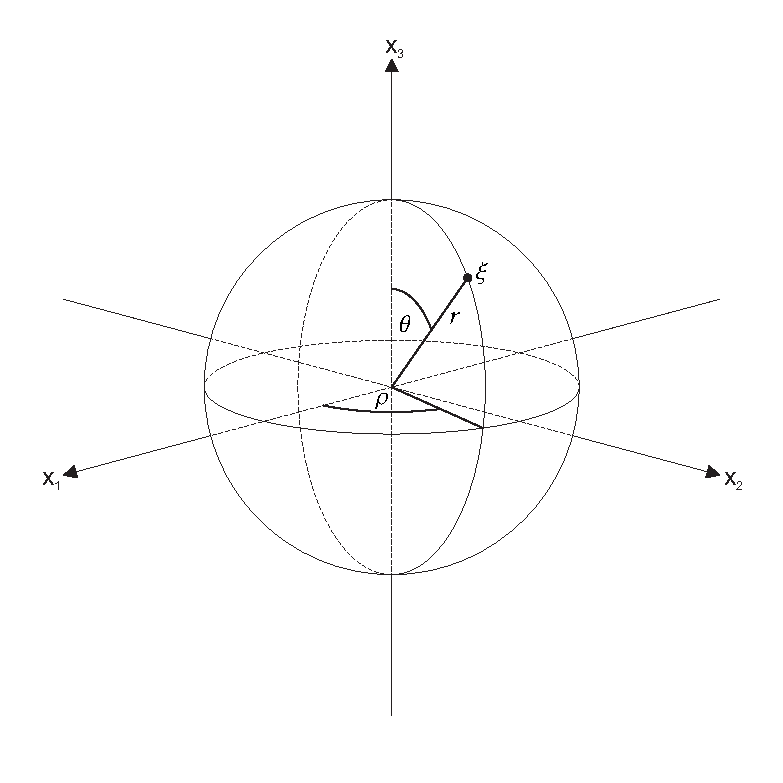
\includegraphics[height=12cm,width=12cm]{images/sphere}
  \caption{The spherical coordinate system in $\R^3$. Every point $\xi$ on a
  sphere with radius $r$ around the origin can be uniquely described by the
  angles $\theta$, $\rho$, and the radius $r$. For $\theta = 0$ or
  $\theta = \pi$ the point $\xi$ coincides with the North or the South
  pole, respectively.}
  \label{sphere}
\end{figure}

We continue our notes on notation by letting $\jkS^m$ be the $m$-th unit
sphere embedded into $\R^{m+1}$, i.e.
\begin{equation}
  \nonumber
  \jkS^m := \jkSetV{\jkSX \in \R^{m+1}}{|}{\jkNorm{\jkSX}_2=1}.
\end{equation}
In subsequent chapters, only $\jkSS$ will be of interest for us.
Therefore, we also use abbreviations like \emph{sphere},
\emph{2-sphere}, or \emph{unit-sphere}, when we refer to $\jkSS$.
The restriction to the unit-sphere further implies $r=1$ for every
point $\jkSX \in \jkSS$. So we identify $\jkSX$ with the vector
$\jkPar{\theta,\rho}^{\text{T}}$, neglecting the fixed radius.

The following easy to prove lemma gives a reformulation of the
standard scalar product in $\R^3$ for spherical coordinates on the
unit sphere.

\begin{lemma}
  Let $\jkSX = \jkPar{\theta,\rho}^{\text{T}}$, $\jkSY = \jkPar{\theta',\rho'}^{\text{T}} \in
  \jkSS$ and $\alpha$ be the angle spanned by the origin and the points $\jkSX$, $\jkSY$.
  Then the standard scalar product
  $\jkScalProd{\jkSX}{\jkSY}_{\jkSS} = \cos\left(\alpha\right)$ is given by
  \begin{equation}
    \nonumber
    \jkFun{\cos}{\alpha} = \cos\theta\cos\theta' +
    \sin\theta\sin\theta'\jkFun{\cos}{\rho-\rho'}.
  \end{equation}
\end{lemma}

\begin{proof}
  Using equation
  \ref{Basics.NotationalConventions.CartesianSphericalCoordinatesIdentity}
  immediately yields the statement.
\end{proof}

Finally, we denote by $\jkFun{\text{Hom}_n}{\R^3}$ the space of
\emph{homogeneous polynomials} of degree $n \in \NZ$ in $\R^3$,
comprising all polynomials $Q_n$ that fulfil $\jkFun{Q_n}{\alpha
x} = \alpha^n \jkFun{Q_n}{x}$ for arbitrary $\alpha \in \R$, $x
\in \R^3$. A subspace of $\jkFun{\text{Hom}_n}{\R^3}$ is defined
by
\begin{equation}
  \jkFun{\text{Harm}_n}{\R^3} = \jkSetV{Q_n \in \jkFun{\text{Hom}_n}{\R^3}}{|}{\jkFun{\jkPar{\Delta_x Q}}{x}=0,\ x \in
  \R^3},
\end{equation}
namely the room of \emph{harmonic homogeneous polynomials} of
degree $n$, where $\Delta_x$ denotes the Laplace-operator
\begin{equation}
  \Delta_x = \frac{\partial^2}{\partial x_1^2} + \frac{\partial^2}{\partial x_2^2} +
  \frac{\partial^2}{\partial x_3^2}.
\end{equation}
Furthermore, the relations
\begin{equation}
  \jkFun{\dim}{\jkFun{\text{Hom}_n}{\R^3}} = \frac{(n+1)(n+2)}{2}\
  \text{and}\ \jkFun{\dim}{\jkFun{\text{Harm}_n}{\R^3}} = 2n+1
\end{equation}
hold (for a proof see \cite{freeden:1998}, Chapters 2.2 and 2.3).
To keep it short, we write $\jkFun{\text{Harm}_n}{\jkSS}$ and mean
the restriction $\left.\jkFun{\text{Harm}_n}{\R^3}\right|_{\jkSS}$
of $\jkFun{\text{Harm}_n}{\R^3}$ to the sphere $\jkSS$.

\subsection{Legendre Polynomials}
Having mentioned some basic agreements, we now introduce the set
of orthogonal Legendre polynomials, the closely related associated
Legendre functions, and discuss their properties. Based one this
foundation, we describe the function space of spherical harmonics
and how it is related to spherical approximation. The reason, why
we set so great store by these topics, is that they not only have
a strong relation to theoretical physics and represent classical,
fundamental methods of spherical approximation, but further build
a mathematical framework for treatments of the following chapters.

Orthogonal polynomials in common, play a great role in
approximation theory. For spherical settings, especially Legendre
polynomials are vital. Not surprisingly, there exists a great
number of characterizations in the literature. In most cases, they
are derived by the \emph{Gram-Schmidt orthonormalization process},
starting with the monomials $\jkEncl{\{}{t^i}{\}}_{i \in \N_0}$
with respect to the inner product
\begin{equation}
\label{LengendreFunctionsAndSphericalHarmonics.LegendreFunctions.ScalarProduct}
  \jkScalProd{f}{g} := \int_{-1}^{1} \jkFun{f}{t}\jkFun{g}{t}\:dt,
\end{equation}
where $f,g : \jkInterv{[}{-1}{1}{]} \mapsto \R$. At variance with
this definition, we use a denotation that yields a different
normalization.

\begin{definition}
  \label{LengendreFunctionsAndSphericalHarmonics.LegendrePolynomials.Definition}
  For $m,n \in \N_0$, the functions $P_n : \jkInterv{[}{-1}{1}{]} \mapsto \R$ with
  \begin{enumerate}
  \item
    $P_n \in \Pi_n$,
  \item
    $\int_{-1}^{1} \jkFun{P_m}{t} \jkFun{P_n}{t} \: dt = \delta_{m,n}$,
  \item
    $\jkFun{P_n}{1} = 1$,
  \end{enumerate}
  are called \textbf{Legendre polynomials}.
\end{definition}

The above definition makes only sense, if every of those
polynomials does not have a zero at $t = 1$. This can be seen from
the corresponding \emph{Rodrigues}-formula:
\begin{equation}
  \nonumber
  \jkFun{P_n}{t} =
  \frac{1}{2^nn!}\frac{d^n}{dt^n}\jkPar{\jkPar{t^2-1}^n}.
\end{equation}
The expression $\jkPar{t^2-1}^n$ represents a polynomial of degree $2n$ with
two $n$-fold zeros at $t = \pm 1$. Each differentiation step adds a new zero in
the interval $\jkInterv{(}{-1}{1}{)}$ and reduces the order of the initial
zeros by one. The final step then makes these zeros disappear, which finally
justifies Definition
\ref{LengendreFunctionsAndSphericalHarmonics.LegendrePolynomials.Definition}.


Many other independent representations are also available. We only propound an
additional recurrence relation in form of the corresponding \emph{three-term
recursion}, which can be obtained for every set of orthogonal polynomials:
\begin{equation}
  \nonumber
  \jkPar{n+1}\jkFun{P_{n+1}}{t} = \jkPar{2n+1}t\jkFun{P_{n}}{t} -
  n\jkFun{P_{n-1}}{t},\ n \in \N.
\end{equation}
For a collection of further representations, we refer the reader
to \cite{conrad:2001} (Section 2.4.1) again.

An interesting property of Legendre polynomials is that for $n$
towards infinity and applied to an argument of the form
$\cos\theta$, they can be approximated by a simple cosine
function, as long, as $\theta$ is restricted to an interval
$\jkInterv{[}{\epsilon}{\pi-\epsilon}{]}$, with $\epsilon > 0$.
This will allow for an investigation of their asymptotic behavior
with regard to the zeros. The following theorem states this famous
result by Laplace, but we omit the proof here.

\begin{theorem}
  \label{LengendreFunctionsAndSphericalHarmonics.LegendrePolynomials.Approximation}
  Let $n \in \N$ and $\theta \in \jkInterv{[}{\epsilon}{\pi-\epsilon}{]}$,
  $\epsilon > 0$. Then the following equation holds:
  \begin{equation}
  \nonumber
    \jkFun{P_n}{\cos \theta} = \sqrt{\frac{2}{\pi n \sin \theta}}
    \jkFun{\cos}{\jkPar{n + \frac{1}{2}}\theta - \frac{\pi}{4}} +
    \jkO{n^{-3/2}}.
  \end{equation}
\end{theorem}

\begin{remark}
  Since the zeros of the Legendre polynomials asymptotically behave like those
  of a cosine, they approach an equidistant distribution in the interval
  $\jkInterv{[}{0}{\pi}{]}$ with respect to $\theta$. This fact will be of use
  in the next chapter.
\end{remark}

Of equal importance is the next characteristic, concerning the power series
\begin{equation}
\label{LengendreFunctionsAndSphericalHarmonics.LegendrePolynomials.PowerSeries}
  \jkFun{\phi}{h} := \sum_{n = 0}^{\infty} \jkFun{P_n}{t} h^n,\ t \in
  \jkInterv{[}{-1}{1}{]},
\end{equation}
which is absolutely and uniformly convergent for $h \in
\jkInterv{(}{-1}{1}{)}$ and features an interesting, yet very
simple representation.

\begin{theorem}
  For all $t \in \jkInterv{[}{-1}{1}{]}$ and $h \in
  \jkInterv{(}{-1}{1}{)}$,
  the identity
  \begin{equation}
  \label{LengendreFunctionsAndSphericalHarmonics.LegendrePolynomials.SeriesExpansion}
    \sum_{n = 0}^{\infty} \jkFun{P_n}{t} h^n = \frac{1}{\sqrt{1-2ht+h^2}}
  \end{equation}
  holds.
\end{theorem}

\begin{proof}
  We give an outline of a proof from \cite{freeden:1998}. First, by differentiation with
  respect to $h$, one gets, after comparing coefficients in line with Equation
  \eqref{LengendreFunctionsAndSphericalHarmonics.LegendrePolynomials.PowerSeries},
  the differential equation
  \begin{equation}
  \nonumber
    \jkPar{1+h^2-2ht}\jkFun{\phi'}{h} = \jkPar{t-h}\jkFun{\phi}{h}.
  \end{equation}
  Under the initial condition $\jkFun{\phi}{0}=1$, this equation yields the
  unique solution
  \begin{equation}
  \nonumber
    \jkFun{\phi}{h}=\frac{1}{\sqrt{1+h^2-2ht}}.
  \end{equation}
\end{proof}

\begin{corollary}
  \label{LengendreFunctionsAndSphericalHarmonics.AssociatedLegendreFunctions.PoissonKernel.Corollary}
  For all $t \in \jkInterv{[}{-1}{1}{]}$ and $h \in \jkInterv{(}{-1}{1}{)}$ it holds
  \begin{equation}
    %\label{LengendreFunctionsAndSphericalHarmonics.AssociatedLegendreFunctions.PoissonKernel}
    \sum_{n=0}^{\infty} \jkPar{2n+1} \jkFun{P_n}{t} h^n =
    \frac{1-h^2}{\jkPar{1-2ht+h^2}^{3/2}}.
  \end{equation}
\end{corollary}

\begin{proof}
  Since the series from Equation
  \eqref{LengendreFunctionsAndSphericalHarmonics.LegendrePolynomials.PowerSeries}
  is differentiable for all $h \in \jkInterv{(}{-1}{1}{)}$, we get
  \begin{equation}
    \label{LengendreFunctionsAndSphericalHarmonics.LegendrePolynomials.DifferentiatedSeriesExpansion}
    \sum_{n = 1}^{\infty} n\jkFun{P_n}{t} h^{n-1}  =
    \frac{h-t}{\jkPar{1+h^2-2ht}^{3/2}}.
  \end{equation}
  Now, using Equations
  \eqref{LengendreFunctionsAndSphericalHarmonics.LegendrePolynomials.SeriesExpansion}
  and
  \eqref{LengendreFunctionsAndSphericalHarmonics.LegendrePolynomials.DifferentiatedSeriesExpansion},
  it follows
  \begin{gather}
    \begin{split}
    \nonumber
        \sum_{n=0}^{\infty} \jkPar{2n+1} \jkFun{P_n}{t} h^n = &
        \sum_{n=0}^{\infty} \jkFun{P_n}{t} h^n + 2h\sum_{n=1}^{\infty} n \jkFun{P_n}{t} h^{n-1}\\
      = & \frac{1}{\sqrt{1-2ht+h^2}} - \frac{2h^2-2ht}{\jkPar{1+h^2-2ht}^{3/2}}\\
      = & \frac{1+h^2-2ht}{\jkPar{1-2ht+h^2}^{3/2}} - \frac{2h^2-2ht}{\jkPar{1+h^2-2ht}^{3/2}}\\
      = & \frac{1-h^2}{\jkPar{1-2ht+h^2}^{3/2}}.
    \end{split}
  \end{gather}
\end{proof}

\begin{remark}
  \label{LengendreFunctionsAndSphericalHarmonics.AssociatedLegendreFunctions.PoissonKernel.Remark}
  When the restriction $h \in \jkInterv{(}{0}{1}{)}$ is applied, the function
  $G_h:\jkInterv{[}{-1}{1}{]} \rightarrow \R$, with
  \begin{equation}
  \nonumber
    \jkFun{G_h}{t} := \frac{1-h^2}{\jkPar{1-2ht+h^2}^{3/2}},
  \end{equation}
  is called \textbf{Poisson kernel}. In Chapter \ref{SphericalBasisFunctions},
  this function will play a major role when we deal with approximation of data on
  the sphere. For the moment, we refer to Figure
  \ref{LengendreFunctionsAndSphericalHarmonics.LegendrePolynomials.Figure.PoissonKernel}
  for a visual impression and take notice of the fact that the parameter $h$
  allows us to control, how much the function's energy is concentrated around
  $t = 1$.
\end{remark}

\subsection{Associated Legendre Functions}

The Legendre polynomials can be generalized. This is done by the
following definition.

\begin{definition}
  Let $n,k \in \N_0$ with $k \le n$. The functions $P_n^k : \jkInterv{[}{-1}{1}{]} \rightarrow
  \R$, given by
  \begin{equation}
    \nonumber
    \jkFun{P_n^k}{t} := \jkPar{\frac{\jkPar{n-k}!}{\jkPar{n+k}!}}^{1/2}
    \jkPar{1-t^2}^{k/2} \frac{d^{k}}{dt^{k}} \jkFun{P_n}{t},
  \end{equation}
  are called \textbf{associated Legendre functions}.
\end{definition}

Associated Legendre functions can be characterized in ways similar
to those for Legendre polynomials, for instance by the
corresponding Rodrigues-formula or a differential equation. They
play an important role in the definition of spherical harmonics.
Note that for $k = 0$, the associated Legendre functions turn out
to be Legendre polynomials.

Similarly, these functions also obey an orthogonality property
with respect to the scalar product from Equation
\eqref{LengendreFunctionsAndSphericalHarmonics.LegendreFunctions.ScalarProduct},
if $k$ is fixed.

\begin{theorem}
\label{LengendreFunctionsAndSphericalHarmonics.AssociatedLegendreFunctions.Orthogonality}
  Let $k,m,n \in \N_0$, $k \le \min\jkEncl{\{}{m,n}{\}}$. Then the associated
  Legendre functions fulfil
  \begin{equation}
  \nonumber
    \int_{-1}^{1} \jkFun{P_{m}^{k}}{t} \jkFun{P_{n}^{k}}{t}\;dt =
    \frac{2}{2n+1}\delta_{m,n}.
  \end{equation}
\end{theorem}

The proof is rather complicated and can be found in
\cite{conrad:2001}, Section 2.4.2.

\subsection{Associated Legendre Polynomials}

\subsection{Spherical Harmonics}
\label{LegendreFunctionsAndSphericalHarmonics.SphericalHarmonics}
In this section, we will review a classical method for spherical
approximation, namely the approximation in the function space of
spherical harmonics. This type of functions is motivated by
problems, which yield partial linear differential equations of
second order.

At first, we recall Laplace's differential equation in $\R^3$ formulated in
Cartesian coordinates,
\begin{equation}
  \nonumber
  \Delta f = \frac{\partial^2f}{\partial x_1^2} + \frac{\partial^2f}{\partial
  x_2^2} + \frac{\partial^2f}{\partial x_3^2} = 0.
\end{equation}
This equation can also be rewritten in spherical coordinates, if
$f$ is restricted to a two-dimensional sphere. The transformation
is complex, but can be performed with elementary operations. We
exclude the details here and show the result directly,
\begin{equation}
  \label{SphericalHarmonics.LaplaceEquation.SphericalCoordinates}
  \Delta f = \frac{\partial^2 f}{\partial r^2} + \frac{2}{r}\frac{\partial f}{\partial
  r} + \frac{1}{r^2 \sin \theta}\frac{\partial}{\partial \theta}\jkPar{\sin \theta \cdot \frac{\partial f}{\partial
  \theta}} + \frac{1}{r^2 \sin \theta}\frac{\partial^2}{\partial \rho^2} = 0.
\end{equation}
The solution can be determined with an approach based on
separation. The sought solution $f$ is written as the product of
three functions, $f = f_r f_\rho f_\theta$, which only depend on
$r$, $\theta$, and $\rho$ respectively. Then, Equation
\eqref{SphericalHarmonics.LaplaceEquation.SphericalCoordinates}
can be rewritten and split up into three equations, each one
containing exactly one variable that can be solved independently
of each other. Again, the calculations necessary are beyond the
scope of this text. The interested reader might want to read
\cite{conrad:2001}, Section 3.1, for a complete derivation of the
solution. For the part depending on $r$, the solution
\begin{equation}
  \nonumber
  f_r(r) := \alpha r^n,
\end{equation}
with $r \in \R^{+}$, arbitrary $n \in \N_0$, and fixed $\alpha \in
\C$, is derived from the linear differential equation with
non-constant coefficients
\begin{equation}
  \label{SphericalHarmonics.DifferentialEquation.r}
  r^2f_r'' + 2rf_r' - \lambda f_r = 0.
\end{equation}
Here, $\lambda$ is a real valued constant. Equation
\eqref{SphericalHarmonics.DifferentialEquation.r} is of the \emph{Euler type}
and can be solved with a well known method. The solution $f_\rho$ for the
$\rho$ part can also be derived with elementary calculations from the equation
\begin{equation}
  \nonumber
  f_{\rho}'' + \mu f_{\rho} = 0,
\end{equation}
where $\mu \in \R$. The solutions are complex exponentials
\begin{equation}
  \nonumber
  \jkFun{f_{\rho}}{\rho} := \beta e^{ik\rho},
\end{equation}
with $\rho \in \jkInterv{[}{0}{2\pi}{)}$, $k \in \Z$ and a fixed $\beta \in
\C$. For the remaining part depending only on $\theta$, the calculations yield
a differential equation, which is characteristic for the associated Legendre
functions, here applied to an argument of the form $\cos\theta$:
\begin{equation}
  \nonumber
  \jkFun{f_{\theta}}{\cos \theta} := \gamma \jkFun{P_{n}^{\jkAbs{k}}}{cos
  \theta},\ \theta \in \jkInterv{[}{0}{\pi}{]}, \gamma \in \C.
\end{equation}
It remains to be noticed that the values $n$ and $k$ are fixed
among the different solutions $f_r$, $f_{\rho}$ and $f_{\theta}$.
After combination, these results gather in a set of functions in
spherical coordinates, all solving equation
\eqref{SphericalHarmonics.LaplaceEquation.SphericalCoordinates}.
For our considerations, we let $r = 1$ and introduce an additional
scaling factor depending on $n$, resulting in functions $Y_{n,k}$
with

\begin{eqnarray*}
  & Y_{n,k}: \jkInterv{[}{0}{\pi}{]}\times\jkInterv{[}{0}{2\pi}{)} \rightarrow
  \C,\\
  & \jkFun{Y_{n,k}}{\theta,\rho} := \sqrt{\frac{2n+1}{4\pi}} \jkFun{P_{n}^{\jkAbs{k}}}{\cos \theta}
  e^{ik\rho}.
\end{eqnarray*}

It is behind the scope of this text to prove further properties of
this functions and delve into details. But to understand their
importance in the context of spherical approximation, we want to
present the most significant facts. Surprisingly at first, it can
be shown that the solutions $Y_{n,k}$ are contained in the space
of homogeneous harmonic polynomials over $\jkSS$, namely
$\jkFun{\text{Harm}_n}{\jkSS}$, as stated by the following result.

\begin{theorem}
  The functions $Y_{n,k}$ with $n \in \N_0$, $k = -n,\dots,n$ fulfil
  \begin{equation}
  \nonumber
    Y_{n,k} \in \jkFun{\text{Harm}_n}{\R^3}.
  \end{equation}
\end{theorem}

Due to the separability of the functions $Y_{n,k}$, it is not
difficult to prove that they also fulfil orthogonality conditions
with respect to the scalar product
$\jkScalProd{\cdot}{\cdot}_{\jkSS}$. Due to the orthogonality of
the complex exponentials with respect to the standard scalar
product in $\mathbb{L}^2_{2\pi}$, the orthogonality for a fixed
$n$ can be shown:
\begin{equation}
\label{LengendreFunctionsAndSphericalHarmonics.SphericalHarmonics.Orthogonality1}
\jkScalProd{Y_{n,j}}{Y_{n,k}}_{\jkSS} = \frac{2n+1}{2}
\delta_{j,k} \int_{0}^{\pi} \jkFun{P_n^{\jkAbs{j}}}{\cos\theta}
\jkFun{P_n^{\jkAbs{k}}}{\cos\theta} \sin\theta\: d\theta.
\end{equation}
If we now define $\mathcal{H}_n$ to be
$\text{Harm}_n\jkPar{\jkSS}$, it is not difficult to prove that
for every $n \in \N_0$, the set
\begin{equation}
  \nonumber
  \jkSetV{Y_{n,k}}{|}{-n \le k \le n}
\end{equation}
forms an orthonormal basis of $\mathcal{H}_n$, since $\dim \mathcal{H}_n =
2n+1$.

If we use the orthogonality of the associated Legendre functions
from Theorem
\ref{LengendreFunctionsAndSphericalHarmonics.AssociatedLegendreFunctions.Orthogonality},
one can see from Equation
\eqref{LengendreFunctionsAndSphericalHarmonics.SphericalHarmonics.Orthogonality1}
that the stronger condition
\begin{equation}
  \nonumber
  \jkScalProd{Y_{m,j}}{Y_{n,k}}_{\jkSS} = \delta_{m,n}\delta_{j,k}
\end{equation}
holds. This means that the spaces $\mathcal{H}_n$ are orthogonal
to each other and makes clear that a set of the form
$\jkSetV{Y_{n,k}}{|}{n = 0,\dots,N,\ -n \le k \le n}$ with $N \in
\N_0$ is an orthonormal basis for the space
$\bigoplus_{n=0}^{N}\mathcal{H}_n$.

\begin{definition}
  The function space $\bigoplus_{n=0}^{N}\mathcal{H}_n$ is called
  the space of \textbf{spherical harmonics} of degree $N$.
\end{definition}

\begin{theorem}
  For every $N \in \N$, the set $\jkSetV{Y_{n,k}}{|}{n = 0,\dots,N,\ -n \le k \le n}$ forms an
  orthonormal basis of the space of spherical harmonics of degree
  $N$.
\end{theorem}

For practical concerns, spaces of this form seem not to be very
useful. The restriction to homogeneous and harmonic polynomials
might exclude various functions from being as well representable,
as in $\jkFun{\Pi_n}{\jkSS}$. The following theorem dispels this
apprehension by showing that the mentioned spaces are identical.

\begin{theorem}
  Every function from the space of polynomials with maximum degree $N \in \N$,
  restricted to the sphere $\jkSS$, can be represented as a sum of spherical
  harmonics of maximum degree $N$, hence
  \begin{equation}
  \nonumber
    \jkFun{\Pi_N}{\jkSS} = \bigoplus_{n=0}^{N}\mathcal{H}_n.
  \end{equation}
\end{theorem}

The last result shows clearly, what a fundamental role spherical
harmonics play for approximation on the sphere. This scheme is
today widely used for a wide range of problems. Spherical
harmonics can be seen as a somewhat natural extension of the
Fourier basis in $\mathbb{L}^2_{2\pi}$ to the sphere. The
latitudinal part is represented by the well known complex
exponentials, while for the longitudinal portion, the associated
Legendre functions come to play. A different aspect is that
spherical harmonics also inherit some well known negative
properties of the participating functions. For rough data, the
result of the approximation with spherical harmonics often shows
unwanted ripple structures near sharp deviations in the input
data. There are several applications, where the given experimental
data just share these conditions. In the following chapters, we
will take a look at a different approach which can prevent this
behavior.

At last, we will now state the well-known addition theorem of
spherical harmonics that relates basis functions of
$\mathcal{H}_n$ and Legendre-polynomials.

\begin{theorem}
\label{AdditionTheorem}
  For every $\jkFun{L^2}{\jkSS}$ orthonormal basis
  $\jkSet{Y_{n,k}}_{k=-n}^{n}$ of $\mathcal{H}_n$, it holds
  \begin{equation}
  \nonumber
    \sum_{k=-n}^{n} \jkFun{Y_{n,k}}{\jkSX}
    \overline{\jkFun{Y_{n,k}}{\jkSY}} =
    \frac{2n+1}{4\pi}\jkFun{P_n}{\jkScalProd{\jkSX}{\jkSY}_{\jkSS}}.
  \end{equation}
\end{theorem}

The result of this important theorem will be employed in the
following chapter.

\subsection{Discret Spherical Fourier Transform}

\section{Fast Spherical Fourier Transform}

\subsection{Fast Legendre Transform}

\subsection{Fast Reconstruction on special grids}

\subsection{Fast reconstruction at arbitrary nodes}

\section{Fast Inverse Spherical Fourier Transform}

\subsection{Fast Legendre Transform Reviewed}
In this section we represent the FLFT algorithm as a linear operator, hence a matrix, that acts on a vector of Fourier-coefficients. So let $M \in \N$ be a fixed bandwidth and as usual $t := \lceil\log_2{M}\rceil$, $N := 2^t$. Furthermore let  $-M \le n \le M$ be fixed. The FLFT can be represented as a matrix $\mb{T} \in \R^{(N+1) \times (N+1)}$ that multiplied with a vector $\mb{a} = \left(a_0^n,a_1^n,\dots,a_N^n\right)^T \in \C^{N+1}$ of Fourier coefficients gives a vector $\mb{g}_n = \left(g_0^n,g_1^n,\dots,g_{2N-1}^n\right) \in \C^{2N}$ containing the Chebyshev coefficients of the polynomial $g_n$: $$\mb{g_{n}} = \mb{T} \; \mb{a}.$$ For the sake of simplicity we omit the fact that $a_{k}^n = 0$ for $k < n$ or $k > M$. Clearly, this can be exploited in the algorithm to save some computational steps.

Since the FLFT algorithm is asymptotically faster than the naive evaluation of the polynomial $g_{n}$ at the Chebyshev nodes, this implies a factorization of $\mb{T}$ into sparse matrices. This factorization can be derived directly from the algorithm already presented and will later be used to construct an algorithm for the transposed problem. In general the FLFT consists of $t+1$ steps so that $\mb{T}$ can be written as $$\mb{T} = \mb{T}_{t} \: \cdot \:  \mb{T}_{t-1} \dots \mb{T}_{1} \: \cdot \:  \mb{T}_{0} \text{, with } \mb{T}_{\tau} \in \left\{\begin{array}{l@{\quad \text{if} \quad}l} \R^{2N \times (N+1)} & \tau = 0, \\ \R^{2N \times 2N} & 1 \le \tau < t, \\ \R^{(N+1) \times 2N} & \tau = t. \end{array}\right.$$

\subsubsection{The First Step}

The first step consists in converting each Fourier-coefficent $a_{k}^n$ into a polynomial of degree at most 1 in Chebyshev representation $\mb{a}_{k}^{(0)} \in \C^2$ so that the result $\mb{a^{(0)}}$ is a vector of length $2N$, hence $$ \mb{a}_{k}^{(0)} = \mb{e}_{1} a_{k}^n,\quad \text{with } \mb{e}_{1} = \left(\begin{array}{l}1\\0\end{array}\right).$$
The last polynomial $\mb{a}_{N}^{(0)}$ is mapped to the preceeding two polynomials by means of the three term recurrence for associated Legendre Functions, i.e. $\mb{a}_{N}^{(0)} = \left(\alpha x + \beta\right)\mb{a}_{N-1}^{(0)} + \gamma \mb{a}_{N-2}^{(0)}$. Following this, $\mb{T}_{0}$ can be written as
$$\left(\mb{I}_{N} \otimes \mb{e}_{1},\;\mb{\tilde{e}}\right),$$ 
where $\mb{\tilde{e}} = \left(0,0,\dots,0,\gamma, 0, \beta,\alpha\right)^T \in \R^{2N}.$

\subsubsection{Cascade Summation}

Steps $1$ to $t-1$ represent the cascade summation that is applied to associated Legendre functions. In each round, half of the the functions is eliminated by mapping them to the remaining functions. Therefore the vector is divided into consecutive blocks, each consisting of four polynomials representing the factors in front of each function. Each polynomial is represented by its vector of Chebyshev coefficients of length $2^{\tau}$. In every block, the first and the second polynomial remain unchanged. The third and the fourth polynomial are multiplied with a matrix $\mb{U}$ that transforms them into a representation in terms of the first two functions. Following this, the output contains only half of the polynomials compared to the input vector, but due to the multiplication with $\mb{U}$ the degree might double each time so that twice the space is needed to store the Chebyshev coefficients. So in total the result vector still has length $2N$. For each step $1 \le \tau < t$ and for each block $$\mb{\tilde{a}}_{l}^{(\tau-1)} := \left(\mb{a}_{4l}^{(\tau-1)},\mb{a}_{4l+1}^{(\tau-1)},\mb{a}_{4l+2}^{(\tau-1)},\mb{a}_{4l+3}^{(\tau-1)}\right)^T \text{, where } 0 \le l < 2^{t-\tau-1},$$ we need to keep the first two polynomials but with their vectors zero-padded up to twice the length. Furthermore, the multiplication with the matrix $\mb{U}$ acts on the third and fourth polynomial.
Correspondingly, each block $\mb{\tilde{a}}_{l}^{(\tau-1)}$ is multiplied by a matrix $\mb{V}_{\tau}^l := \left[\mb{Z_{\tau}},\mb{U}_{\tau}^l\right]$, with
$$\mb{Z}_{\tau} := \left(\begin{array}{cccc} \mb{I}_{2^{\tau}} & 0\\ 0 & 0 \\ 0 & \mb{I}_{2^{\tau}} \\ 0 & 0 \end{array}\right) \in \R^{2^{\tau+2} \times 2^{\tau+1}},\ \mb{U}_{\tau}^l \in \R^{2^{\tau+2} \times 2^{\tau+1}}.$$
%Correspondingly, this can be written as the product 
%$$\mb{ZP}_{\tau} \; \mb{\tilde{a}}_{l}^{\tau-1} \text{, with } \mb{ZP}_{\tau} := \left(\begin{array}{cccc} \mb{I}_{2^{\tau}} & 0 & 0 & 0\\ 0 & 0 & 0 & 0 \\ 0 & \mb{I}_{2^{\tau}} & 0 & 0 \\ 0 & 0 & 0 & 0 \end{array}\right) \in \R^{2^{\tau+2} \times 2^{\tau+2}}.$$ 
%The multiplication with the matrix $\mb{U}$ that acts on the third and fourth polynomial is written as $\mb{U}_{\tau}^l \; \mb{\tilde{a}}_{l}^{\tau-1}$ where the matrix can be factorized as follows:
The matrix $\mb{U}_{\tau}^l$ can be factorized as follows:
$$ \mb{U}_{\tau}^l = \mb{D}_{\tau}^{II} \; \cdot \; \mb{S}_{\tau} \; \cdot \; \mb{P}_{\tau}\left(2^{\tau + 1}l+1\right) \; \cdot \; \mb{D}_{\tau}^{III}  \in \R^{2^{\tau+2} \times 2^{\tau+1}}$$
where we define
\begin{eqnarray*}
  \mb{D}_{\tau}^{II} & := & \mb{I}_{2} \otimes \left(\mb{\tilde{D}}_{2^{\tau+1}} \mb{\tilde{C}}_{2^{\tau+1}}\right) \in \R^{2^{\tau+2} \times 2^{\tau+2}},\\
  \mb{S}_{\tau} & := & \mb{I}_2 \otimes \left[\begin{array}{cc}\mb{I}_{2^{\tau+1}},\mb{I}_{2^{\tau+1}}\end{array}\right] \in \R^{2^{\tau+2} \times 2^{\tau+3}},\\
  \mb{P}_{\tau}(c) & := & \text{diag}\left(\gamma_{c}^n \mb{P}_{2^{\tau}-2}^n(c+1),\gamma_{c}^n \mb{P}_{2^{\tau}-1}^n(c+1),\right.\\
    & & \left. \mb{P}_{2^{\tau}-1}^n(c), \mb{P}_{2^{\tau}}^n(c)\right) \in \R^{2^{\tau+3} \times 2^{\tau+3}},\\
  \mb{D}_{\tau}^{III} & := &\mb{I}_{2} \otimes \left(\left(\mb{I}_{2} \otimes \mb{\tilde{C}}^T_{2^{\tau+1}}\right)\mb{Z}_{\tau}\right) \in \R^{2^{\tau+3} \times 2^{\tau+1}}.
\end{eqnarray*}   
This interpretation corresponds directly to the algorithm implemented. The matrix $\mb{D}_{\tau}^{III}$ realizes first the zero-padding of the two polynomials ($\mb{Z}$), second the evaluation of the polynomials at the Chebyshev nodes ($\mb{\tilde{C}}^T$) and finally a duplication of the result vector in order to permit multiplication with two different associated Legendre functions for each polynomial. The matrix $\mb{P}_{\tau}(c)$ contains the associated Legendre polynomials of the matrix $U_{2^{\tau}-1}^n(\cdot,2^{\tau+1}l+1)$ also evaluated at the Chebyshev nodes on its main diagonal. Therefore a multiplication with this matrix realizes a pointwise multiplication of the zero-padded and evaluated polynomials. For each of the two rows of $U_{2^{\tau}-1}^n(\cdot,2^{\tau+1}l+1)$, two of the results of the previous step are summed by the following multiplication with the matrix $\mb{S}_{\tau}$. Finally, the matrix $\mb{D}_{\tau}^{II}$ transforms the newly formed polynomials back into Chebyshev coefficients.

From the factorization a more compact representation can be obtained, so that $\mb{U}_{\tau}^l$ can be written as
\begin{equation}
\label{UCompact}
\mb{U}_{\tau}^l = 
\left(\begin{array}{lclrcr}
\mb{\mb{\tilde{D}}_{2^{\tau+1}}\tilde{C}}_{2^{\tau+1}} & \gamma_{c}^n & \left(\right. & \mb{P}_{2^{\tau}-2}^n(c+1) \mb{\tilde{C}}^T_{2^{\tau+1}} Z_{1} & + & \mb{P}_{2^{\tau}-1}^n(c+1) \mb{\tilde{C}}^T_{2^{\tau+1}} Z_{2} \left.\right) \\
\mb{\mb{\tilde{D}}_{2^{\tau+1}}\tilde{C}}_{2^{\tau+1}} & & \left(\right. & \mb{P}_{2^{\tau}-1}^n(c) \mb{\tilde{C}}^T_{2^{\tau+1}} Z_{1} & + & \mb{P}_{2^{\tau}}^n(c) \mb{\tilde{C}}^T_{2^{\tau+1}} Z_{2} \left.\right)
\end{array}\right)
\end{equation}
%So for each block $l$, a multiplication with a matrix $\mb{V}_{\tau}^l  \in \R^{2^{\tau+2} \times 2^{\tau+2}}$ is applied where
%$$ \mb{V}_{\tau}^l = \left[\mb{ZP},\mb{U}_{\tau}^l\right].$$ 
The complete round can then be represented as $$\mb{T}_{\tau} = \text{diag}\left(\mb{V}_{\tau}^0,\mb{V}_{\tau}^1,\dots,\mb{V}_{\tau}^{2^{t-\tau-1}-1}\right).$$

\subsubsection{The Last Step}
The last step consists of calculating the polynomial $g_{n} = \mb{a}_{0}^{(t-1)} P_{0}^{|n|} + \mb{a}_{1}^{(t-1)} P_{1}^{|n|}$ in Chebyshev representation. Since 
$$P_{0}^n(x) = \frac{\left( \left( 2n \right) ! \right)^{1/2}}{2^n n!},\ P_{1}^n(x) = \left(\alpha_{0}^nx + \beta_{0}^n\right)P_{0}^n(x)$$ we can use 
$$xT_{0}(x) = T_{1}(x),\ xT_{k}(x) = \frac{1}{2}\left( T_{k+1}(x) + T_{k-1}(x) \right)$$ to write
$$ \mb{g_{n}} = \gamma_{0}^n \left( \mb{I}_{N+1} \mb{a}_{0}^{(\tau-1)} + \left( \alpha_{0}^n\mb{W}_{N+1} + \beta_{0}^n\mb{I}_{N+1} \right) \mb{a}_{1}^{(\tau-1)} \right)$$
Depending on $n \in \N_{0}$, we can distinguish three cases:
\begin{description}
  \item[n odd:] In this case, $\alpha_{0}^n = 0$ and $\beta_{0}^n = 1$ so that $\mb{T}_{\tau}$ can be written as $$\mb{T}_{\tau} = \gamma_{0}^n \left[ \mb{I}_{N+1}, \mb{I}_{N+1} \right].$$
  \item[n = 0:] Here it holds, $\alpha_{0}^n = 1$ and $\beta_{0}^n = 0$ and we get $$\mb{T}_{\tau} = \gamma_{0}^n \left[ \mb{I}_{N+1}, \mb{W}_{N+1} \right].$$
  \item[n even, n > 0:] Now $\alpha_{0}^n = -1$ and $\beta_{0}^n = 1$ which results in $$\mb{T}_{\tau} = \gamma_{0}^n \left[ \mb{I}_{N+1}, \mb{I}_{N+1} - \mb{W}_{N+1} \right].$$
\end{description}
where we define
$$
\mb{W}_{n} :=
\left(
\begin{array}{ccccccc}
  0 & \frac{1}{2} &             &                           \\
  1 &           0 & \frac{1}{2} &                           \\
    & \frac{1}{2} &           0 & \ddots                    \\
    &             &      \ddots & \ddots      & \frac{1}{2} \\
    &             &             & \frac{1}{2} &           0
\end{array}
\right)
\in \R^{n \times n}.
$$

\subsection{The Adjoint Operator}
Following the factorization of $\mb{T}$ given in the previous section, one obtains easily the adjoint operator which is paramount for an implementation of xxx: 
$$\mb{T}^H = \mb{T}_{0}^H \; \cdot \; \mb{T}_{1}^H \dots \mb{T}_{t-1}^H \; \cdot \; \mb{T}_{t}^H.$$ For $\tau = 0$ and $\tau = t$ we obtain immediatly
$$ \mb{T}_{0}^H = \left( \begin{array}{c} \mb{I}_{N} \otimes \mb{e}_{1}^T\\ \mb{\tilde{e}}^T \end{array}\right), \mb{T}_{t}^H = \gamma_{0}^n \left\{\begin{array}{l@{\quad \text{if} \quad}l} 
 \left[ \begin{array}{c} \mb{I}_{N+1} \\ \mb{I}_{N+1} \end{array} \right] & \text{n odd},\\[2ex]
 \left[ \begin{array}{c} \mb{I}_{N+1} \\ \mb{T}_{N+1}^T \end{array} \right] & \text{n = 0},\\[2ex]
 \left[ \begin{array}{c} \mb{I}_{N+1} \\ \mb{I}_{N+1} - \mb{T}_{N+1}^T \end{array} \right] & \text{n even, n > 0}.
\end{array}\right.$$
Using xxx we get for the rest of the steps $\mb{T}_{\tau}$, $1 \le \tau \le t-1$
\begin{eqnarray*}
 \mb{T}_{\tau}^H & = & \text{diag}\left({\mb{V}_{\tau}^0}^H,{\mb{V}_{\tau}^1}^H,\dots,{\mb{V}_{\tau}^{2^{t-\tau-1}-1}}^H\right),\\
 {\mb{V}_{\tau}^l}^H & = & \left[ \begin{array}{c} \mb{Z}^H \\ { \mb{U}_{\tau}^l}^H \end{array} \right],\\
 {\mb{U}_{\tau}^l}^H & = &
   \left(
     \begin{array}{rlllr}
        \gamma_{c}^n & \left(\right. Z_{1}^T \mb{\tilde{C}}_{2^{\tau+1}} \mb{P}_{2^{\tau}-2}^n(c+1)   & + & Z_{2}^T \mb{\tilde{C}}_{2^{\tau+1}} \mb{P}_{2^{\tau}-1}^n(c+1)
         & \left.\right) \mb{\tilde{C}}_{2^{\tau+1}}^T \\
        & \left(\right. Z_{1}^T \mb{\tilde{C}}_{2^{\tau+1}} \mb{P}_{2^{\tau}-1}^n(c) & + & Z_{2}^T \mb{\tilde{C}}_{2^{\tau+1}} \mb{P}_{2^{\tau}}^n(c) & \left.\right) \mb{\tilde{C}}_{2^{\tau+1}}^T
     \end{array}
   \right).
\end{eqnarray*}
 

\clearpage

\begin{thebibliography}{99}

  \bibitem{conrad:2001}
  {\sc Matthias Conrad,}
  \newblock{\em Approximation und Multiskalenzerlegung auf der Sph�re,}
  \newblock{Diploma thesis, Institute for Applied Mathematics, University of Hamburg, 2001}
   
\end{thebibliography}

\end{document}